\subsection {Introduction}
%\addcontentsline{toc}{section}{Introduction}
The Leibniz Institute for the Social Sciences (GESIS) as the biggest service provider for the social sciences in europe.
Our self-imposed goal is to offer the best support for social scientiststs in each step of there professional work.\footnote{Overview of GESIS services: \url{https://www.gesis.org/en/services}}
Scientists and analysts often face the problem of finding interesting research datasets and identifying who else used the data, in which research fields, and how the data has been analyzed from a methodological perspective.
In the step of searching relevant publications and datasets we provide an integrated search\footnote{GESIS search \url{search.gesis.org}}.
Here we integrate not only references to publications and dataset.
We also provide references to variables and questions and instruments and tools into one search portal.
To connect entries from this variety of data types we developed a set of tools.
On the one hand those tools are supporting manual annotators to identify connections between those types.
On the other hand we consider automatic approaches which, for example are able to detect references to datasets or survey data from given full text publications.
The development of the latter tools was carried out as part of the InFoLis project.\footnote{\url{https://www.gesis.org/en/research/external-funding-projects/archive/infolis-i-and-ii}}.
Because of the history of reseach of our institution regarding the task (e.g.\cite{boland2012identifying,ghavimi2016semi}) we were happy to note the ambitions of the Coleridge Initiative to evolve this research field with the help of the Rich Context Competition\footnote{\url{https://coleridgeinitiative.org/richcontextcompetition}} (RCC).
A Competitions to automate the process of interlinking publications, research methods and research fields.

This chapter describes our approaches, techniques, and used additional data used for our participation in the RCC.

% Old intro for CompetitionTo address these problems, the Coleridge Initiative organized the Rich Context Competition
%The competition invited international research teams to develop text analysis and machine learning tools that can discover relationships between research datasets, methods, and fields in scientific literature.
%The competition took place between October 2018 and February 2019 and included two phases\footnote{\url{https://coleridgeinitiative.org/richcontextcompetition\#competitionschedule}}.
%The first phase was open for all teams which have submitted a letter of intent.
%Teams are then provided with a corpus of social science publications to develop and train machine learning algorithms for automatic research dataset, methods and field detection and linking. 
%More concretely, one major subtask consisted of linking dataset mentions to a given set of around 10,000 dataset descriptions from the ICPSR’s research data index.\footnote{\url{https://www.icpsr.umich.edu/index.html}}
%Only the best four teams from the first phase are invited to the second phase of the competition and asked to discover research datasets, methods, and fields in a larger corpus of social science publications. 
%More about the type of scientific publications can be found in Section~\ref{subsec:rcc-corpus}.

%The Rich Context Competition\footnote{\url{https://coleridgeinitiative.org/richcontextcompetition}}(RCC) is organized by the Coleridge Initiative and targets both US and international researchers. The main goal of the competition is to automate the discovery of research datasets and the associated research methods and fields in social science publications. 
%task is to extract information from full texts to be able to create a network of publications, datasets and research methods.

%\subsection{Task Definition of the RCC}
%In both competition phases the task was to submit a software package which is able to process PDF (respectively extracted raw text) on the Servers of the organizers.
%The software have to be able to extract dataset mentions, research methods and research fields from the given publication. More about the type of scientific publications can be found in Section~\ref{subsec:rcc-corpus}.
%In the first phase additional the software has to be able to link dataset mentions to a given set of around 10,000 dataset descriptions originate from ICPSR\footnote{\url{https://www.icpsr.umich.edu/icpsrweb/ICPSR/}} research data index.


\subsubsection{Non-technical overview}

\begin{itemize}
    \item Usage of external data
    \item Supervised machine learning Approaches
    \item Problem of Training data: weak supervision
\end{itemize}


% Literature Review


\subsubsection{General Approach and Software Components}
%\subsection{Our Approach on a technical perspective}
The central tasks in the RCC are the extraction of dataset mentions from text. 
Even so, we considered the discovery of research methods and research fields important.
To this end, we decided to follow a module-based approach. Users could choose to use each specific module solely or as parts of a data processing pipeline.
Figure~\ref{figure:pipeline} shows an overview of modules developed  and their dependencies . Here, the upper three modules (which are in gray) describe the pre-processing steps (cf. Section~\ref{sec:prepro}).
The lower four modules (blue) are used to generate the output in a pre-specified format. 

The pre-processing step consists of extracting metadata and pure text from PDF documents. The extraction itself is done using the Cermine Tool\footnote{\url{https://github.com/CeON/CERMINE}} which returns a Journal Article Tag Suite\footnote{\url{https://jats.nlm.nih.gov}}(Jats) XML document. Then, in a second step,
text, metadata and references are extracted. The output of the pre-processing is then used by the software modules responsible for tackling the individual sub-tasks, i.e., discovering research datasets (cf. Section~\ref{sec:dataset-extraction}), methods (cf. Section~\ref{section:research_method_extraction}) and fields (cf. Section~\ref{section:field_classification}).


%After pre-processing, a Named Enity Recognition module is used to find data set mentions. The training corpus and process is described in Section~\ref{sec:dataset-extraction}.

%In the next step, we combine all recognized mentions for each publication and compare these mentions to the metadata from `data_sets.json`.
%The mentions are used in an interim format which also persists the sentence of each mention. Also, all years are extracted from theses sentences
%and used in the retrieval process. After retrieving the best matching results, theses are returned in the target format for `data_set_citation.json`.

%For identifying research fields, we trained a classifier on abstracts and metadata crawled from the Social Science Open Access Repository\footnote{\url{https://www.ssoar.info}} (SSOAR). We used the OAI-API for this and the crawler is delivered in the module.
%We tried different classifiers and selected the best performing one, a [fasttext]() classifier, i.e. a neural net based approach with a high performance.


\begin{figure}[t]
    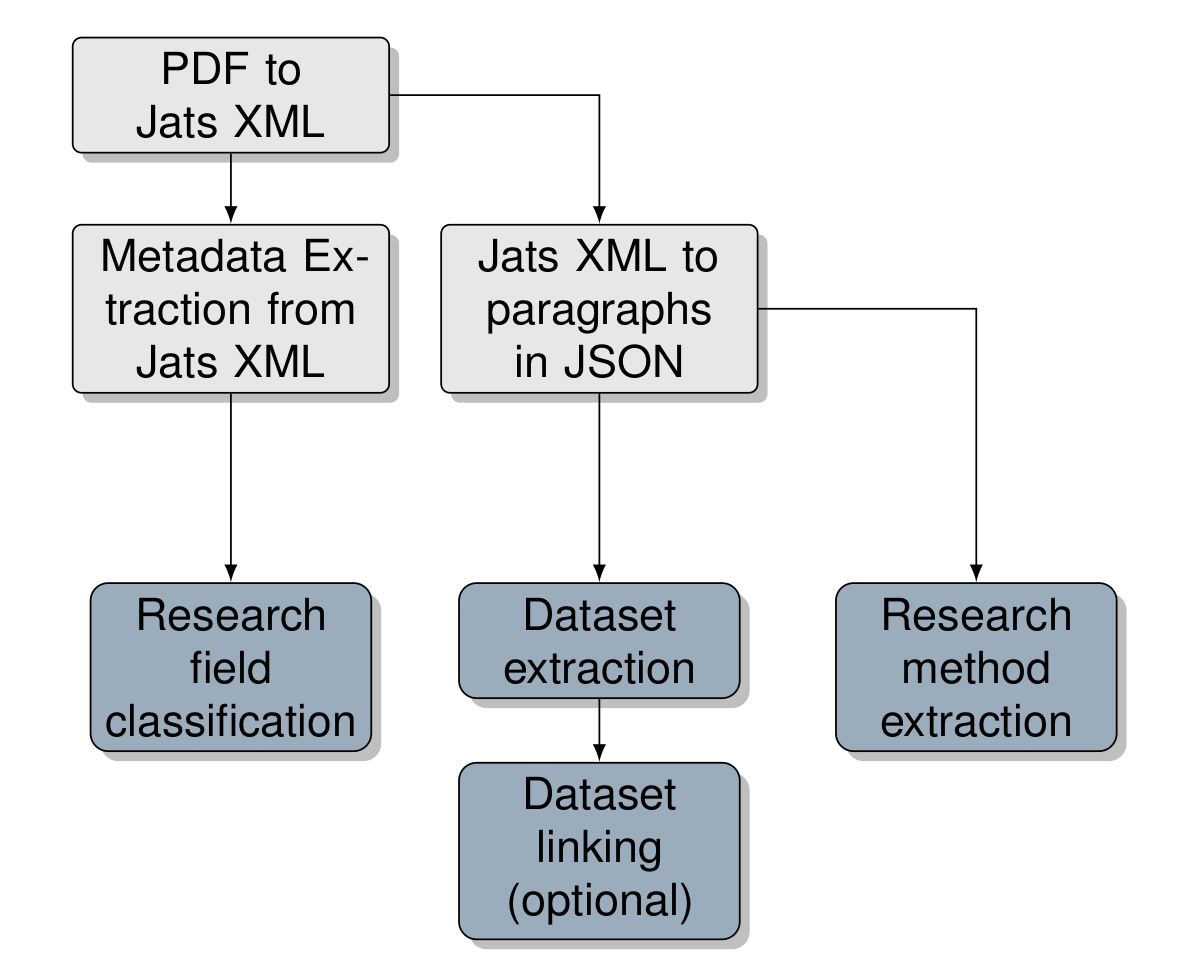
\includegraphics[width=0.47\textwidth]{figures/information-flow.png}
    \caption{An overview of the individual software modules described in this document and their dependencies. 1- Gray: Our pre-processing pipeline. 2- Blue: three main tasks of the RCC.}
    \label{figure:pipeline}
\end{figure}

\subsubsection{First Phase Feedback}
After the first phase, each team received feedback from the organizers of the RCC.
The feedback is two folds and consists of a quantitative and qualitative evaluation. Unfortunately, the quantitative assessment showed our algorithms did not perform well regarding precision and recall metrics. In contrast to this, our approach has been found convincing regarding the quality of results. The qualitative feedback was from a random sample of ten documents given to four judges.
Judges are then asked to manually extract dataset mentions and calculate the overlap between their dataset extractions and the output of our algorithm.
Other factors that judges took into consideration are specificity, uniqueness, and multiple occurrences of dataset mentions.
As for the extraction of research methods and fields, no ground truth has been provided; these tasks were evaluated against the judges' expert knowledge.
Similarly to the extraction of dataset mentions, specificity and uniqueness have been considered for these two tasks.
The feedback our team received acknowledged the fact that no ground truth has been provided and our efforts regarding the extraction of research methods and fields.
%Feedback by RCC
%Section~\ref{} gives detailed overview of data provided by the RCC and additional data sources used in our approach. :o .
